\documentclass[a4paper,12pt]{report}
\setcounter{secnumdepth}{5}
\setcounter{tocdepth}{3}
\newcounter{ZhRenew}
\setcounter{ZhRenew}{1}
\newcounter{SectionLanguage}
\setcounter{SectionLanguage}{1}
\input{/usr/share/latex-toolkit/template.tex}
\begin{document}
\title{天文學}
\author{沈威宇}
\date{\temtoday}
\titletocdoc
\chapter{天文學(Astronomy)}
\section{宇宙}
\subsection{天體系統}
\textbf{宇宙}:包含暗物質、暗能量、一般物質、一般能量等。
\begin{itemize}
\item \textbf{本超星系團}
\begin{itemize}
\item \textbf{本星系群}
\begin{itemize}
\item \textbf{銀河系}:為棒旋星系,即中間具有由恆星聚集組成短棒形狀的螺旋星系。銀河系的中心稱銀心,是一個超大質量黑洞,被命名為人馬座A*。銀河系直徑約100 kly,棒半長度約1至5 kpc,太陽距離銀心約25至28 kly。銀河系有數個螺旋臂,有程度不一的不規則性。銀河系的盤面被一個扁球狀的銀暈包圍著,估計直徑在250,000至400,000光年,其中有許多球狀星團。銀道坐標系以太陽為原點,極軸通過銀心。太陽系大約每2.25—2.5億年在軌道上繞行銀心一圈,可稱為一個銀河年。一般認為銀河系在約136億年前形成。
\begin{itemize}
\item \textbf{恆星系統}:如太陽系。
\item \textbf{星雲}:星際氣體與塵埃形成的雲狀天體,與恆星誕生相關者有反射星雲(反射鄰近恆星的星光)、暗星雲(濃密的星雲遮蔽後方的星光)與發射星雲(星雲內部恆星發光),與恆星死亡相關者有行星狀星雲。
\item \textbf{星團}:一群聚集的星星,分為球狀與疏散星團,前者較後者恆星較多、單一恆星質量較小、恆星較老、重元素含量較高,前者分布於銀暈,後者分布於銀河盤面。
\item\textbf{其他星際物質}
\end{itemize}
\item \textbf{仙女座星系}
\item \textbf{大麥哲倫星系}
\item \textbf{小麥哲倫星系}
\item \textbf{其他成員星系}:星系依據外觀分為螺旋、棒旋、橢圓、不規則等四大類,是構成宇宙的基本單位。
\end{itemize}
\item \textbf{其他星系群}:星系群與星系團同等級,惟成員數不超過100個者稱星系群,否則稱星系團。
\item \textbf{室女座星系團}
\item \textbf{其他星系團}
\end{itemize}
\item \textbf{后髮座超星系團}
\item \textbf{其他超星系團}
\end{itemize}
\subsection{宇宙年表(Chronology of the Universe)}
\bctf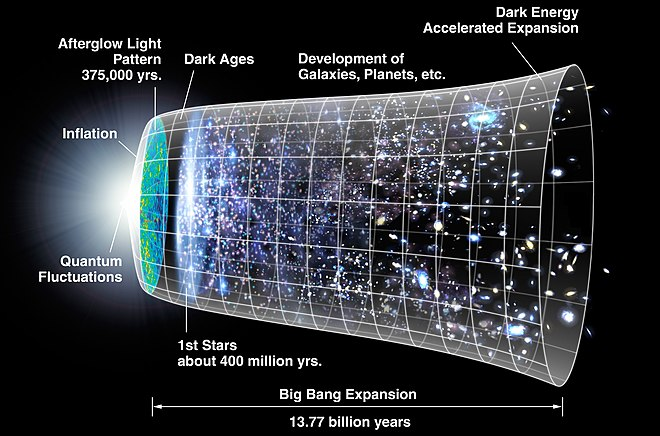
\includegraphics[width=0.9\textwidth]{宇宙年表.jpg}\efct
\subsubsection{普朗克時期(Planck Epoch)}
\begin{itemize}
\item \textbf{時間範圍}:大爆炸(Big Bang,又稱大霹靂)後 \(10^{-43}\) 秒以內
\item \textbf{特點}:最早有意義的時間。奇(異)點(singularity)指宇宙誕生時的極端高密度、高溫狀態。在這個奇點,所有的物質和能量都集中在一個無限小的點。現有物理學理論無法描述這個時期的狀態。所有基本力(引力、電磁力、強力、弱力)可能統一為一個單一的力。通常認為,引力的量子效應在這個時間尺度上主導著物理相互作用。
\end{itemize}
\subsubsection{大統一時期(Grand Unification Epoch)}
\begin{itemize}
\item \textbf{時間範圍}:大爆炸後 \(10^{-43}\) 秒到 \(10^{-36}\) 秒
\item \textbf{特點}:溫度下降到 \(10^{32}\text{K}\) 足以使重力和其他基本力分離。強力和電弱力仍然統一,稱大統一力,可能由 X 和 Y 玻色子介導。
\end{itemize}
\subsubsection{電弱時期(Electroweak Epoch)}
\begin{itemize}
\item \textbf{時間範圍}:大爆炸後 \(10^{-36}\) 秒到 \(10^{-12}\) 秒
\item \textbf{特點}:大爆炸後 \(10^{-36}\) 秒到 \(10^{-32}\) 秒為暴脹時期(Inflationary Epoch),宇宙經歷指數級膨脹,體積迅速增加,宇宙溫度從 \(10^{28}\text{K}\) 下降到 \(10^{22}\text{K}\),強力與電弱力分離,宇宙溫度仍然極高,基本粒子開始形成,W 和 Z 玻色子及希格斯玻色子可能由 X 和 Y 玻色子衰變而成。
\end{itemize}
\subsubsection{夸克時期(Quark Epoch)}
\begin{itemize}
\item \textbf{時間範圍}:大爆炸後 \(10^{-12}\) 秒到 \(10^{-6}\) 秒
\item \textbf{特點}:宇宙充滿夸克、反夸克和膠子,溫度足以阻止夸克結合成質子和中子。
\end{itemize}
\subsubsection{強子時期(Hadron Epoch)}
\begin{itemize}
\item \textbf{時間範圍}:大爆炸後 \(10^{-6}\) 秒到 1 秒
\item \textbf{特點}:宇宙冷卻到 \(10^{10}\text{K}\),使夸克能夠發生夸克-強子轉變,結合形成強子(如質子和中子)。
\end{itemize}
\subsubsection{輕子時期(Lepton Epoch)}
\begin{itemize}
\item \textbf{時間範圍}:大爆炸後 1 秒到 10 秒
\item \textbf{特點}:宇宙冷卻到 \(10^{9}\text{K}\),大多數強子和反強子相互湮滅,反夸克可能消失,輕子(如電子、緲子和微中子)主導宇宙,重力減慢宇宙的膨脹,微中子與物質解耦,形成宇宙微中子背景。
\end{itemize}
\subsubsection{光子時期(Photon Epoch)}
\begin{itemize}
\item \textbf{時間範圍}:大爆炸後 10 秒到 37 萬年
\item \textbf{特點}:大多數輕子和反輕子相互湮滅,正電子可能消失。光子主導宇宙能量,電子和核子結合形成中性原子,光子得以自由運動,形成宇宙微波背景(Cosmic Microwave Background,CMB)輻射。宇宙微波背景輻射,是宇宙學中大霹靂遺留下來的熱輻射,充滿整個宇宙並隨宇宙膨脹而紅移,現今其頻率和2.725K的黑體輻射相同,屬微波範圍,故又稱3K背景輻射,於1964年被發現。普通物質粒子與光和輻射耦合,而暗物質粒子開始建構非線性結構,如暗物質暈。由於帶電電子和質子阻礙光的發射,宇宙變成了超熱的發光霧。
\end{itemize}
\subsubsection{黑暗時代(Dark Age)}
\begin{itemize}
\item \textbf{時間範圍}:大爆炸後 37 萬年到 10 億年
\item \textbf{特點}:宇宙微波背景輻射的溫度從約 4,000 K 冷卻至約 60 K,光子僅來源於中性氫的解耦和偶爾釋放的光子,宇宙呈現黑暗,宇宙開始由物質主導,宇宙的膨脹因為重力而減慢。
\end{itemize}
\subsubsection{再電離時期(Reionization Epoch)}
\begin{itemize}
\item \textbf{時間範圍}:大爆炸後 1.5 億年到 10 億年
\item \textbf{特點}:第一代恆星(第三族恆星)的結構開始形成,其輻射能量重新電離宇宙中的中性氫,使分裂回自由電子和質子的等離子體。大爆炸後約 4 億年,第一代恆星形成。
\end{itemize}
\subsubsection{星系形成和演化(Galaxy Formation and Evolution)}
\begin{itemize}
\item \textbf{時間範圍}:大爆炸後 10 億年至今
\item \textbf{特點}:物質在引力的影響下繼續聚集在一起,形成星系、星系團/群和超星系團。宇宙膨脹持續。早期形成第二族恆星,而後形成第一族恆星。
\end{itemize}
\subsubsection{暗能量主導時代(Dark Energy–Dominated Era)}
\begin{itemize}
\item \textbf{時間範圍}:大爆炸後 98 億年到至今
\item \textbf{特點}:宇宙加速膨脹,推測是由暗能量驅動。暗能量現在被認為是宇宙中最大的單一組成部分,約占物理宇宙整個質能的 68.3\%。
\end{itemize}
\subsubsection{現在}
距離大爆炸 $13.799 \pm 0.021 \times 10^9$ 年。
\subsubsection{宇宙的終極命運(Ultimate Fate of the Universe)}
\begin{itemize}
\item 大冰凍(Big Freeze)/熱寂(Heat Death):持續膨脹導致宇宙達到最大熵的狀態,接近絕對零度,其中一切都均勻分佈,並且不存在能量梯度。
\item 大撕裂(Big Rip):哈伯常數在有限時間內增加到無限大。宇宙中的物質,都被膨脹逐漸撕裂。
\item 大緊縮(Big Crunch):宇宙膨脹的力量最終被引力所克服,宇宙開始收縮,最終所有物質重新集中到一個極端密度的點,類似於大爆炸的初始奇點。
\item 大反彈(Big Bounce):宇宙經歷大緊縮後,再次膨脹,可能與大爆炸的過程類似,但這一理論尚未被廣泛證實。
\end{itemize}
\subsection{哈伯–勒梅特定律(Hubble-Lemaître law)/哈伯定律(Hubble's law)}
\subsubsection{哈伯常數(Hubble's constant)}
定義哈伯常數$H$為
\[v=Hd\]
其中$v$是距離地球$d$的星系遠離地球的速率。

$H$常見單位為 km s$^{-1}$ Mpc$^{-1}$。
\subsubsection{減速參數(deceleration parameter)}
哈伯常數的值隨著時間$t$變化取決於無因次的減速參數$q$
\[q=-1-H^{-2}\dv{H}{t}\]
\begin{itemize}
\item $q>1$:宇宙收縮。
\item $q=0$:宇宙不收縮亦不膨脹。
\item $1>q>0$:宇宙減速膨脹。
\item $q=0$:宇宙等速膨脹,有$H = \frac{1}{t}$,其中$t$是自大霹靂以來的時間。
\item $0>q$:宇宙加速膨脹。
\item $0>q>-1$:宇宙加速但次指數膨脹。現在測得$q$值約-0.5。
\item $q=-1$:宇宙指數膨脹。
\item $-1>q$:宇宙超指數膨脹。
\end{itemize}
\subsubsection{哈伯時間/哈伯年齡/哈伯期}
定義宇宙的哈伯時間為$\frac{1}{H}$。

目前估計宇宙年齡(age of the universe)與$\frac{1}{H}$相去不遠。
\section{恆星}
\subsection{距離單位}
\subsubsection{天文單位(Astronomical Unit)}
\begin{itemize}
    \item 舊定義:地球與太陽的平均距離
    \item 新定義:149,597,870,895.265908536440公尺
\end{itemize}
\subsubsection{秒差距(Parsec,pc)}
\begin{itemize}
    \item 約3.26光年、206,000天文單位或31兆公里。
    \item 舊定義:等腰三角形中1天文單位的底邊的對角為1角秒時的股長。
    \item 新定義:$\frac{648000}{\pi}$天文單位。
\end{itemize}
\subsubsection{光年(Light year, ly)}
真空光速乘以一年,約9.46$\times$10$^{15}$ m。
\subsection{星等}
\subsubsection{星座}
星座是指天上一群恆星的組合,如西方的星座與中國的星宿。1930年,國際天文學聯合會為了統一繁雜的星座劃分,用精確的邊界把天空分為88個正式的星座,使天空多數恆星都屬於某一特定星座。這些正式的星座大多都以古希臘傳統星座為基礎。通常某星座中最亮者稱某座\text{\textalpha}星、次亮者稱某座\text{\textbeta}星。
\subsubsection{視星等(Apparent Magnitude, $m$)}
\begin{itemize}
    \item 西元前二世紀依巴谷(Hipparchus)把天上最亮的20顆恆星定為1等星,人眼可見的最暗星定為6等星,之間分為2至5等,等級數字愈大亮度愈暗。
    \item 現定義:
    \[
    m = -2.5 \log \left( \frac{F}{F_0} \right)
    \]
    其中:
    \begin{itemize}
        \item $m$:視星等(等)
        \item $F$:亮度($\text{lx} = \text{cd}/\text{m}^2$)
        \item $F_0$:參考零點亮度 $\approx 10^{-5.672} \text{ lx}$,一般以標準光源計算相對亮度,即定織女星為0等計算其他天體的視星等
    \end{itemize}
\end{itemize}
\subsubsection{絕對星等(Absolute Magnitude, $M$)}
將天體移至10秒差距時呈現的視星等。\\
絕對星等愈大,發光強度愈大。\\
若不考慮星光與大氣吸收等影響,視星等$m$、絕對星等$M$與距離$d$(單位秒差距)的關係為:
\[m-M=5\log(d)-5.\]
\subsection{恆星的光譜}
\subsubsection{星色}
\bctf\icg[width=0.7\tw]{Wiens.png}\cpt{4C, 2006.}\efct
星色:指天體輻射在可見光區段中輻射峰值頻率考慮其與地球相對運動的都卜勒效應後呈現的顏色。\\
黑體輻射遵守普朗克定律與維恩位移定律,能量密度峰值之頻率與功率密度均與絕對溫度正相關。像太陽一樣表面溫度約6000K的天體,不考慮都卜勒效應,能量峰值頻率落在藍光和綠光之間。\\
行星之顏色無法推知表面溫度,因為其顏色係與表面化學組成有關,故火星因地表有大量氧化鐵而呈紅色。
\subsubsection{恆星光譜類型(The Classification of Stars/Stellar Classification)}
\bctf\icg[width=0.9\tw]{Stellar_Classification_Chart.png}\cpt{Pablo Carlos Budassi, 2020.}\efct
Most stars are currently classified under the Morgan–Keenan (MK) system using the letters O, B, A, F, G, K, and M, a sequence from the hottest (O type) to the coolest (M type). Each letter class is then subdivided using a numeric digit with 0 being hottest and 9 being coolest (e.g., A8, A9, F0, and F1 form a sequence from hotter to cooler). The sequence has been expanded with three classes for other stars that do not fit in the classical system: W, S and C. Some stellar remnants or objects of deviating mass have also been assigned letters: D for white dwarfs and L, T and Y for Brown dwarfs (and exoplanets).
\subsubsection{各波段物質}
\begin{itemize}
\item 熱氣體:已游離的高溫氣體發出X射線。超新星爆炸發出的光可用裸眼看見數週之久。
\item 高溫星:較大、較高溫的恆星發出紫外線。
\item 太陽型恆星:與太陽大小相仿的恆星發出可見光。太陽以黃綠色光輻射最強。
\item 低溫星:較小、較低溫的恆星發出紅外線。
\item 冷氣體:冷到可以讓分子存在的雲氣發出無線電波。
\end{itemize}
\subsubsection{恆星成分}
多數恆星與太陽大氣相似,氫占多數,氦次之,其他較重元素僅占1至4\%。
\subsection{核融合(Nuclear fusion)}
\subsubsection{Proton–proton chain (p-p chain)}
p-p chain 中氫融合為氦的分支為大宗,而後依 H $\rightarrow$ He $\rightarrow$ C $\rightarrow$ O $\rightarrow$  Si $\rightarrow$ Fe 發生。太陽及以下溫度的恆星只能發生 p-p chain 核融合。
\subsubsection{CNO cycle}
以 C12 $\rightarrow$ N13 $\rightarrow$ C13 $\rightarrow$ N14 $\rightarrow$ O15 $\rightarrow$ N15 $\rightarrow$ C12 的 CNO-I cycle 最多,其有氫的參與,並再每次循環產生一個氦。溫度比太陽略大的恆星以 CNO cycle 為主要的核融合。
\subsubsection{Triple-α process}
He $\rightarrow$ Be $\rightarrow$ C 的 triple-α process 發生於溫度遠高於太陽的恆星。
\subsection{赫羅圖}
\subsubsection{赫羅圖(Hertzsprung–Russell diagram, HR diagram, H-R diagram, HRD, HR圖, H-R圖)}
橫軸為表面溫度,低溫在右(對應到光譜類型O-M),縱軸為絕對星等,負在上(對應到對數光度)。
\bct\bfH\ctr\icg[width=0.9\textwidth]{HRD.png}\cpt{Richard Powell. The Hertzsprung Russell Diagram. \href{http://www.atlasoftheuniverse.com/hr.html}{http://www.atlasoftheuniverse.com/hr.html}.}\ef\ect
\subsubsection{主序星(Main Seqence Stars)}
\begin{itemize}
\item 赫羅圖位置:對角線,從左上(高溫、高光度)到右下(低溫、低光度)。
\item 質量分類:小於0.4太陽質量者稱低質量恆星,0.4-8太陽質量者稱中質量恆星,大於8太陽質量者稱高質量恆星。
\item 特徵:約90\%的恆星,包括我們的太陽,都位於這條主序帶上。這些恆星在核心中進行氫的核融合,將氫轉化為氦,釋放出能量。愈靠近左上角的主序星光度愈高、愈偏藍白色、溫度愈高、體積常愈大、質量愈大、氫消耗速率愈大、壽命愈短,因為核融合反應要與重力平衡。這是恆星演化的最長階段,占恆星壽命約九成。主序星中的氫燃燒平衡了重力壓力,使恆星保持穩定。質量較小的紅色主序星低溫黯淡,氫可用數千億年方耗盡,太陽壽命約100億年。
\item 溫度和光度:溫度範圍從幾千度到數萬度K不等,光度跨度很大。
\end{itemize}
\subsubsection{白矮星(White Dwarfs)}
\begin{itemize}
\item 赫羅圖位置:左下角。
\item 中質量恆星形成白矮星:中質量恆星,在紅巨星或紅超巨星階段結束後,外層物質會拋出,核心部分收縮為一顆白矮星,外層物質形成一圍繞白矮星之球狀雲系,稱行星狀星雲。
\item 低質量恆星形成白矮星:低質量恆星,在氫核融合反應結束後,核心塌縮使溫度上升,但仍無法觸發氦融合成碳的反應,成為一顆白矮星。
\item 特徵:恆星演化的最終階段之一,體積非常小但溫度高,炙熱且緻密。它們不再進行核融合,主要由電子簡併壓力支撐。白矮星冷卻至無法發光稱黑矮星,理論上現宇宙年齡不足以形成黑矮星。
\item 溫度和光度:雖然白矮星的溫度高,但它們的光度非常低,因為它們的表面面積很小。
\end{itemize}
\subsubsection{紅巨星(Red Giants)}
\begin{itemize}
\item 赫羅圖位置:右上角。
\item 中質量恆星形成紅巨星:中質量恆星,在氫核融合反應結束後,核心塌縮使溫度上升,觸發氦融合反應,外層膨脹形成紅巨星。中質量恆星僅能進行到氦,最終變成白矮星。
\item 特徵:這些恆星已經耗盡了核心中的氫,開始進行氦融合,進一步形成碳和氧。如果恆星的質量足夠大,會繼續融合更重的元素,導致外層膨脹。紅巨星的半徑非常大,光度也很高,但表面溫度較低,呈現紅色或橙色。
\item 溫度和光度:它們的溫度較低(通常低於4000K),但光度非常高。
\end{itemize}
\subsubsection{超巨星(Supergiants)}
\begin{itemize}
\item 赫羅圖位置:上方。
\item 高質量恆星形成超巨星:高質量恆星,當核心的氫耗盡後,發生類似中質量恆星形成紅巨星的過程,形成超巨星。
\item 紅超巨星:是超巨星的一種,是體積最大的一種恆星,與紅巨星類似。
\item 特徵:超巨星的壽命較短,最終會發生超新星爆炸。
\item 溫度和光度:超巨星的溫度和光度變化很大,溫度可以從幾千度到數萬度K不等,但它們的光度極高。紅超巨星如參宿四(Betelgeuse)。
\end{itemize}
\subsection{星雲假說(Nebular hypothesis)}
是在天體演化學中用以解釋太陽系的形成與演化最被廣泛接受的模型。它提出太陽系是在星雲物質中形成的,繞太陽運行的氣體和塵埃形成了行星。
\subsubsection{星雲(Nebula)/巨分子雲(Giant molecular cloud,GMC)}
恆星間的空間近似真空,僅有一些氣體和塵埃散布其中,稱星際物質。聚集時,形成星雲。星雲主要由九成的氫和百分之九的氦組成,剩下為較重的元素、分子與塵埃。當這些雲在重力上不穩定,物質將在其中凝聚成更小、更緻密的團塊,然後旋轉、坍塌,並可能形成原恆星。
\begin{itemize}
\item 發射星雲:這些星雲內部的高能恆星輻射足夠的能量,使周圍的氣體電離並發出可見光。常見的例子包括獵戶座星雲。
\item 反射星雲:當星雲中的塵埃和氣體反射附近恆星的光線時,形成了反射星雲。這些星雲本身並不發光,常見的例子是昴宿星團附近的星雲。
\item 行星狀星雲:這些星雲是在恆星生命晚期階段,當外層氣體被噴射後形成的。它們通常呈現出圓形或橢圓形,像是行星一般,常見的例子是螺旋星雲。
\item 超新星殘骸星雲:當大質量恆星以超新星的形式爆炸後,其爆炸殘留的氣體與塵埃形成了這類星雲。蟹狀星雲便是其中著名的一個例子。
\item 暗星雲:由於內部物質極為密集,這些星雲會阻擋來自背後的星光,從而呈現出暗斑或陰影的樣貌,如馬頭星雲。
\end{itemize}
\subsubsection{原恆星(Protostar)}
在星際介質中的巨分子雲發生重力塌縮下,氣體和塵埃聚集成團,塌縮的中心區域形成原恆星。這個階段,原恆星的溫度和壓力逐漸升高,足以產生紅外線,但還沒有達到核融合的條件。是恆星形成過程中的早期階段。對一個太陽質量的恆星而言,這個階段至少持續大約10$^5$年。它開始於分子雲核心的密度增加,結束於金牛T星的形成,然後就發展進入主序帶。
\subsubsection{原行星盤(Proplyd)}
星際雲的崩塌並不是完全對稱的,結果是整個系統開始旋轉。角動量守恆使得雲塵和氣體形成一個旋轉的盤狀結構,稱為原行星盤,這解釋了為何太陽系多數行星均接近黃道面。最初非常熱,盤面隨後在所謂的金牛座 T 星階段冷卻,可能形成由岩石和冰組成的小塵埃顆粒,這些顆粒最終可能會凝結成千米大小的星子。太陽星雲的原行星盤約在 46 億年前形成。
\sssc{主序星}
當原恆星進一步塌縮,核心溫度和壓力足夠時(達到約1,000萬度),氫核融合反應開始(將氫轉變為氦),恆星進入主序星階段。可觀察到星雲物質受激發、高溫氣體噴射流與逐漸被吹散。
\subsubsection{恆星系統}
恆星強烈的恆星風和輻射會清除掉原行星盤中剩餘的氣體和塵埃,只留下已經形成的行星、衛星、小行星和彗星等。經過一段時間後,行星軌道逐漸穩定,形成我們現在所看到的成熟恆星系統。
\subsubsection{棕矮星(Brown dwarf)}
如果原恆星的質量大約低於0.08太陽質量,在核心不會點燃正常的核融合反應。重力收縮不足以讓這麼小的原恆星產生足夠的熱,而在核心的溫度達到可以引發核融合反應之前,密度已經達到使原子密集到足以創建量子狀態的電子簡併壓力。由電子簡併壓力所達到的密度和壓力,阻止了物質繼續向核心掉落,使無法形成主序恆星,稱棕矮星,屬於次恆星。
\subsubsection{類地行星}
如果原行星盤夠大,失控的吸積就會開始,塵埃顆粒開始相互碰撞並黏結,導致在 10 萬到 30 萬年的時間內迅速形成月球到火星大小的行星胚胎。在恆星附近,行星胚胎將經歷劇烈合併的階段,產生了一些類地行星,大約需要一億到十億年。
\subsubsection{類木行星}
在強烈的恆星風和高熱下,冰或氣體物質無法存在於靠近恆星的環境,在較外圍以冰的相互吸附為起點,逐漸凝聚再進一步吸附氣體,形成類木行星。
\subsubsection{恆星系統中之小天體}
無法聚集成球形的團塊圍繞恆星公轉,形成恆星系統中之小天體。這些天體質量極小,沒有能力改變自身形狀與化學組成,保存了早期恆星系統形成時的資訊。
\subsubsection{恆星死亡形成星雲}
中、高質量恆星死亡時,會將部分物質拋回太空,包含核融合反應產生的重元素(原子序大於2的元素)。這些星際物質可重新聚集成星雲,如太陽星雲屬之。
\subsubsection{超新星(Supernova)爆炸形成中子星或黑洞}
質量極大的超巨星之核融合達到產生鐵時因該過程吸熱使核心無法再通過核融合反應支持自身重力,結果核心快速塌縮。在這個過程中,核心密度和溫度急劇上升,電子和質子結合形成中子,核心變成一個高度致密的中子星或黑洞。核心塌縮產生的衝擊波反彈回外層,將外層物質以極高的速度拋入太空,形成超新星爆炸。這個過程可以核融合產生比鐵重的元素,釋放出超過億萬顆恆星發光總和的大量能量和光輻射,約持續一秒,使超新星變得極為明亮,短時間內甚至能超過整個星系的光度。
\section{太陽系}
\subsection{太陽(Sun)}
太陽系的中心,是一顆中等大小的恆星,質量約$1.99\times 10^{30} kg$,半徑約$6.95\times 10^5 km$。表面溫度高達攝氏6000度,行核融合並放出輻射,提供了系統中所有天體所需的光和熱。
\sssc{光球(Photosphere)}
是恆星向外輻射出光線的區域,從天體的表面向內延伸,直到氣體變得不透明的區域。
\sssc{日冕(Solar corona)}
是太陽外圍的高溫氣體,溫度遠高於光球層但密度低故光度較光球層低,日全食時、使用日冕儀或以X射線波段觀測可見。

冕洞(Coronal hole)是日冕中因為能量和氣體比平均密度低,而使溫度較低所形成的黑暗區域。
\sssc{太陽黑子(sunspot)}
是太陽光球上的臨時現象,在可見光下呈現比周圍區域黑暗的斑點,由局部高密度的磁性活動抑制了對流的激烈活動造成。太陽黑子數量愈多時,日冕範圍愈大,太陽閃焰發生頻率愈高,太陽表面活動愈頻繁,發出愈多短波輻射與帶電粒子,太陽風愈快速。
\subsubsection{太陽風(Solar wind)}
是太陽外圍大氣流出的超高速電漿流。在太陽日冕層的幾百萬度高溫下,氫、氦為主的原子被等離子化,形成約為質子89\%、$\alpha$粒子10\%、重元素1\%的質量組成。這些帶電粒子運動速度極快,以致不斷有帶電的粒子掙脫太陽的引力束縛,射向太陽的外圍,形成太陽風,以每秒約二百至八百公里的速度向外散逸。

太陽活動較不活躍時,太陽的磁極處附近吹出的太陽風較高速,磁赤道附近吹出的太陽風較低速。

當太陽存在冕洞時,太陽風較高速。

由於太陽的轉動,太陽磁場被太陽風拉扯成螺線形狀。
\sssc{太陽週期(Solar cycle)}
週期約 11 年的太陽表面活動、黑子數量與磁場活動的活躍程度之週期性變化,極大時稱太陽極大期(Solar maximum),極小時稱太陽極小期(Solar minimum)。
\ssc{宇宙射線(Cosmic ray)}
是來自太空穿透力較強且近光速移動的高能粒子,大部分是質子和電子,能量可達$10^20 eV$。
\ssc{日球(Heliosphere)}
在星際媒質(主要是稀薄的氫和氦)中,太陽風因為與宇宙射線相抗衡而吹出一個氣泡狀的日球,為以氫核為主的厚牆。太陽風不能繼續推動星際媒質的地方稱之為日球層頂/頂層(Heliopause),是一堵約一百萬到兩百萬攝氏度、厚度超過10AU的氫氣牆,大約在距太陽120AU處,也通常被認為是太陽系的外邊界。
\subsection{行星(Planet)}
行星是環繞太陽運行的流體靜力平衡形狀天體,且質量夠大足以清除軌道附近的其他天體。太陽系共有八大行星,分為類地行星與類木行星。
\begin{table}[H]
\centering
\begin{tabular}{|c|c|c|}
\hline
\textbf{特色比較} & \textbf{類地行星} & \textbf{類木行星} \\ \hline
距離太陽 & 近 & 遠 \\ \hline
行星軌道間距 & 小 & 大 \\ \hline
體積 & 小 & 大 \\ \hline
質量 & 小 & 大 \\ \hline
主要組成 & 金屬、岩石 & 冰、氣體 \\ \hline
固態表面 & 有 & 沒有 \\ \hline
密度 & 大 & 小 \\ \hline
自轉 & 慢 & 快 \\ \hline
磁場 & 弱 & 強 \\ \hline
行星環 & 沒有 & 有 \\ \hline
衛星 & 少或沒有 & 多 \\ \hline
\end{tabular}
\caption{類地行星與類木行星的比較}
\end{table}\FB
\subsection{矮行星(Dwarf planet)}
矮行星是環繞太陽運行的流體靜力平衡形狀的天體,且質量不夠大不足以清除軌道附近的其他天體。太陽系中國際天文學聯合會認證的矮行星有穀神星、冥王星、鬩神星、妊神星和鳥神星,其中僅穀神星位於火星與木星之間的小行星帶,其餘均位於柯伊伯帶或離散盤。
\subsection{太陽系小天體}
太陽系小天體是環繞太陽運行的天體,且不屬於行星或矮行星。例如小行星與彗星。
\subsubsection{彗星(Comet)}
俗稱掃帚星。彗星係未分化的石頭、金屬、冰和氣體聚集而成。平常是不發光的冰凍體,在接近太陽時,受太陽風和太陽輻射的影響,冰會昇華成氣體,產生慧髮與慧尾。
\begin{itemize}
\item 慧核:主要由塵埃、石塊與固態水、氨、甲烷等構成。彗核本體通常不超過50公里。
\item 慧髮:環繞彗核的雲狀彗髮直徑可達數千到數百萬公里,是受到太陽輻射影響使彗核物質揮發形成。
\item 彗尾:分為始終背向太陽的離子尾,由帶電物質組成,和因為慣性落後離子尾的塵埃尾,顆粒較大,分布較寬。慧尾長度愈接近太陽愈長,可達1 AU以上。
\item 軌道:彗星的軌道通常是偏心率很大的橢圓形。週期小於200年的短週期彗星一般來自柯伊伯帶或離散盤;週期大於200年的長週期彗星一般來自歐特雲。
\end{itemize}
\subsubsection{小行星(Asteroid)}
小行星主要由金屬和岩石組成,通常比較堅硬,不容易揮發。軌道較為圓形,主要集中在火星和木星之間的小行星帶,該處小行星係被太陽和木星拉扯而無法聚集為行星。它們的大小和形狀差異很大,微米至百公里量級都有。
\subsubsection{流星(Meteor)}
\begin{itemize}
\item 流星:隕石灰塵等受地球吸引高速進入大氣層,與大氣摩擦生熱,流星體與周遭氣體因高溫激發放出亮光。
\item 流星雨:地球運行到彗星(或少數為小行星,如雙子座流星雨)所遺留下的碎屑群附近時,吸引大量流星進入大氣層,稱之。一流星雨之軌跡往源頭延伸約可相交於一點,稱輻射點。若輻射點位於某星座區域,則稱該流星雨為該星座流星雨。同一星座流星雨每年約於固定時間再現。
\end{itemize}
\subsection{離太陽由近到遠依序排列}
\begin{itemize}
    \item \textbf{水星(Mercury)}:0.4 AU。類地行星。最接近太陽,沒有大氣層,隕石坑多,表面溫差極大(-200°C~400°C)。
    \item \textbf{金星(Venus)}:0.7 AU。類地行星。擁有約90大氣壓、二氧化碳為主的大氣層,平均表面氣溫約464°C,順時針自轉,自轉週期大於公轉週期,質量與體積略小於地球,反照率高故是地球夜空可見最亮之行星。
    \item \textbf{地球(Earth)}:1.0 AU。類地行星。位於適居帶(Habitable Zone),適居帶是指恆星系統中適合生命居住的區域,理論上表面溫度可以讓水保持液態存在。地球有以下保護,使其利於生物生存:
    \begin{itemize}
    \item 磁場:液態外核產生磁場。磁場阻擋大部分太陽風、宇宙射線等帶電粒子。
    \item 磁層:衝進磁層的帶電粒子大部分會被捕獲在范艾倫輻射帶,高能帶電粒子在其中移動時會放出X射線。
    \item 電離層(增溫層和中性層):吸收短波紫外線及以上頻率之電磁波。太陽活動劇烈時,磁層帶電粒子沿磁場進入兩極大氣層,撞擊高層大氣原子或分子,產生極光。
    \item 平流層:臭氧吸收中長波紫外線。
\item 塵埃與碎屑和空氣粒子摩擦燃燒縮小,少數未盡者稱為隕石。
\item 大氣成分和濃度合宜,使溫室效應適中。
\end{itemize}
    \item \textbf{火星(Mars)}:1.5 AU。類地行星。擁有約0.01大氣壓、二氧化碳為主的大氣層,溫室效應弱,溫差大(-85°C~-5°C),表面有冰和可能有液態水,有似曾經水流之痕跡,自轉軸傾斜25度,有四季變化,自轉週期約24小時,地表有大量氧化鐵故呈紅色。
    \item \textbf{小行星帶(Asteroid Belt)}:火星與木星之間。被認為是太陽系形成過程中被木星引力干擾,未能聚合成行星的剩餘物質,體積約微米至數百公里,其中僅穀神星為矮行星,其餘為小行星。大多數為金屬、岩石組成。
    \item \textbf{木星(Jupiter)}:5.2 AU。類木行星。太陽系質量、體積最大的行星,表面有大紅斑,成分以氫、氦氣體為主。
    \item \textbf{土星(Saturn)}:9.6 AU。類木行星。以其明顯的環系著稱,成分以氫、氦氣體為主,太陽系密度最小的行星。
    \item \textbf{天王星(Uranus)}:19.0 AU。類木行星。自轉軸幾乎平行於公轉平面,因甲烷大氣吸收陽光的紅光而擁有淡藍色的外觀,較木星、土星有更大比例的固態甲烷、氨和水。
    \item \textbf{海王星(Neptune)}:30.0 AU。類木行星。太陽系距離太陽最遠的行星,擁有強烈的風暴,因甲烷大氣吸收陽光的紅光而擁有藍色綠的外觀,較木星、土星有更大比例的固態甲烷、氨和水。
    \item \textbf{柯伊伯帶(Kuiper Belt)}:30-50 AU 接近黃道(地球繞日公轉的軌道)面附近。天體密度高的環狀區域。經典柯伊伯帶天體的軌道為黃道面上的圓形;共振柯伊伯帶天體的軌道與海王星共振,公轉週期與海王星的公轉週期呈現簡單的整數關係。主要為水、甲烷、氨之冰凍天體與岩屑。是短週期彗星發源地。
    \item \textbf{離散盤(Scattered disc)}:同樣在30 AU 之外,一種定義為會接近海王星的天體所運行的軌道區域,故包含柯伊伯帶,另一種定義則去除柯伊伯帶。該處的天體也會受到海王星的影響,且通常偏心率較大且軌道偏離黃道面較多。主要為水、甲烷、氨之冰凍天體與岩屑。是短週期彗星發源地。
    \item \textbf{歐特雲(Oort cloud)}:50-5000 AU。不局限於黃道面而是球狀。主要為水、甲烷、氨之冰凍天體與岩屑。是長週期彗星發源地。
\end{itemize}
\section{地面觀測之參考系}
\subsection{天球(Celestial sphere)}
天球是指以地球為中心,往外無限延伸的假想球體。天球北極向地球觀察,地球自轉、地球公轉、月球自轉、月球公轉都是逆時針。
\bct\bfH\ctr\icg[width=0.9\textwidth]{天球.jpg}\cpt{Tfr000, 2012.}\ef\FB\ect
\subsubsection{赤道坐標系統(Equatorial coordinate system)}
\begin{itemize}
    \item \textbf{天球赤道}(Celestial Equator):天球赤道是與地球赤道平面平行的假想圓。它將天球分成北半球和南半球。
    \item \textbf{赤經}(Right Ascension, RA, α):類似於地球上的經度,赤經是從春分點開始,沿著天球赤道測量的角度,通常以小時、分鐘和秒來表示。
    \item \textbf{赤緯}(Declination, Dec, δ):類似地球上的緯度,赤緯是天體在天球赤道以北為正、以南為負的角度,通常以度、分、秒來表示。
\end{itemize}
\subsubsection{黃道坐標系統(Ecliptic coordinate system)}
\begin{itemize}
    \item \textbf{黃道}(Ecliptic):天球上的黃道是太陽在一年中沿著天球的路徑所形成的圓圈。它與地球的黃道面平行。
    \item \textbf{黃經}(Ecliptic Longitude, λ):沿著黃道測量的角度,從春分點開始計算,通常以度來表示。
    \item \textbf{黃緯}(Ecliptic Latitude, β):天體在黃道平面上的位置,測量天體與黃道平面之間的角度,通常以度來表示。
\end{itemize}
\subsubsection{特殊點}
\begin{itemize}
    \item \textbf{春分點}:太陽春分時在天球上的投影點,位於赤經0h、赤緯0$^\circ$、黃經0$^\circ$、黃緯0$^\circ$。
    \item \textbf{夏至點}:太陽夏至時在天球上的投影點,位於赤經6h、赤緯23.5$^\circ$、黃經90$^\circ$、黃緯0$^\circ$。
    \item \textbf{秋分點}:太陽秋分時在天球上的投影點,位於赤經12h、赤緯0$^\circ$、黃經180$^\circ$、黃緯0$^\circ$。
    \item \textbf{冬至點}:太陽冬至時在天球上的投影點,位於赤經18h、赤緯-23.5$^\circ$、黃經270$^\circ$、黃緯0$^\circ$。
    \item \textbf{天球北極}:赤緯90$^\circ$的點。
    \item \textbf{天球南極}:赤緯-90$^\circ$的點。
\end{itemize}
\subsection{地球觀測者參考系}
\begin{itemize}
\item \textbf{仰角}:仰視目標時,視線與水平線的夾角。
\item \textbf{天頂角}:90$^\circ$ - 仰角。
\item \textbf{中天/中天子午線/子午線}:通過天球北極、觀測者所在位置天頂與天球南極的天球大圓。
\item \textbf{子午面}(Meridian plane):指包含地軸(Earth's axis),即地球自轉軸,與天頂(Zenith)的平面。
\item \textbf{時圈}(Hour circle):指包含地軸與給定興趣點的平面。
\item \textbf{時角}(Hour angle):指子午面和時圈面的兩面角,以東升中的天體為正,西落中的天體為負,即以天球北極向地球觀察所見之順時針為正方向。
\item \textbf{當地時角}(Local hour angle, LHA):指當地觀測到的時角。
\item \textbf{格林威治時角}(Greenwich hour angle, GHA):指本初子午線上觀測到的時角。LHA - GHA = 當地經度。
\item \textbf{恆星時角}(Sidereal hour angle):位於赤經0h在地球上的投影線上的觀察者觀察到的LHA。SHA$_{\text{object}}$ + $\alpha_{\text{object}}$ = 24h。
\end{itemize}
\subsection{不同緯度地面觀測太陽}
\subsubsection{仰角}
北半球觀測者觀察天球北極(即北極星處)的仰角等於當地北緯;南半球觀測者觀察天球南極的仰角等於當地南緯。\\
觀測者觀察春分、秋分太陽在太陽正午(Solar noon),即太陽位於最高點時,即太陽仰角在當日中最大時,太陽之天頂角等於當地緯度。
\subsubsection{太陽的當地時角}
令緯度以北為正,南為負,緯度$\Phi$的觀察者($|\Phi|<23.5^\circ$),在太陽位於赤緯$\Phi$之日的太陽正午觀察太陽,其天頂角為0$^\circ$。
\[\cos \theta _{s}=\sin \alpha _{s}=\sin \Phi \sin \delta +\cos \Phi \cos \delta \cos h\]
其中:${\displaystyle \theta _{s}}\text{是太陽的天頂角}$,${\displaystyle \alpha _{s}}\text{是太陽的仰角}$,${\displaystyle h}\text{是太陽的當地時角}$,${\displaystyle \delta }\text{是太陽的赤緯}$,${\displaystyle \Phi }\text{是當地緯度}$。
\subsection{日}
\subsubsection{周日運動(Diurnal motion)}
指的是天體(如恆星)在一天內相對於天球背景的運動。這種運動是由於地球自轉造成的。地球自西向東自轉,使得天體在天球上看起來從東方升起,向西方落下。這種運動的週期是一天。
\subsubsection{恆星日(Sidereal day)}
恆星日是指地球相對於遠離太陽的恆星(如恆星背景)的一次完整自轉而再次對正同一恆星所需的時間。每個恆星日長度相同,大約為23小時56分鐘4秒,大約比平太陽日少$\frac{1}{365}$。\\
這是測量地球自轉的最精確方式,但不適用於日常時間計算。\\
每個平太陽日恆星提早約4分鐘升起,即向西移動約1度。
\subsubsection{太陽日(Solar day)}
太陽日是地球相對於太陽的一次完整自轉所需的時間。由於地球的公轉軌道並非圓形,太陽日的長度會有所變化。
\subsubsection{平太陽日(Mean solar day)}
平太陽日是指一整個回歸年的太陽日的平均值。大約為24小時,地球約自轉361$^\circ$。
\subsection{月}
\subsubsection{恆星月(Sidereal month)}
恆星日是指月球相對於遠離太陽的恆星(如恆星背景)的一次完整繞地球公轉而再次對正同一恆星所需的時間,約27.32平太陽日。
\subsubsection{朔望月(Synodic/Lunar month)}
從一次新月(朔)經上弦月、滿月(望)、下弦月等,至下一次新月(朔)的時間,約29.5306平太陽日。
\subsubsection{月相盈虧}
月球面向太陽的一面為受光面,地球可見月球受光面之圖形,即月相。
\subsubsection{月球自轉}
月球平均自轉一圈之時間等於一朔望月。
\subsection{年}
\subsubsection{黃道(Ecliptic)}
黃道是地球繞太陽的軌道,在天球上呈現為太陽在一年中圍繞天球運動在背景恆星上描繪出的一條路徑。\\
黃道面與月球公轉軌道面(白道面)夾約5度,故日月蝕非每月可見。
\subsubsection{周年運動(Annual motion)}
指的是太陽在一年內相對於恆星背景的運動。這種運動是由於地球繞太陽公轉造成的。地球每年繞太陽一周,使得太陽在天球上沿著黃道運動。這種運動的週期是一年。地球繞日公轉每天移動大約1度,使得太陽與恆星背景在天球上的相對位置不斷改變,造成恆星每天提早4分鐘出現,一年之後方能在同一時刻看到相同的恆星背景。
\subsubsection{黃道星座(天文)}
黃道處的恆星背景上的星座,自一月太陽位置起隨太陽在黃道上的視運動方向依序為魔羯、寶瓶、雙魚、白羊、金牛、雙子、巨蟹、獅子、室女、天秤、天蠍、蛇夫、人馬。當地球、太陽與某星座略呈直線(太陽在中間)時,稱太陽運行到該星座。春分約在雙魚,夏至約在金牛至雙子,秋分約在室女,冬至約在人馬。
\subsubsection{回歸年(Tropical year)/太陽年(Solar year)}
太陽連續兩次通過春分點所需的時間稱為一個回歸年,長度約365.2422平太陽日。
\subsubsection{地球公轉}
北半球夏至時地球位於遠日點附近,冬至時位於近日點附近。
\subsection{蝕(Eclipse)}
\subsubsection{日蝕}
發生於太陽、月(朔月)與地球成一直線時。由於月球遠近不同和月球偏離日地連線角度,在月球在地球之投影中心位置觀察,有日全蝕、日環蝕與日偏蝕,地球上偏離月球投影中心較遠處亦可見日偏蝕。\\
根據觀測,月球以每年約3.8厘米的速度遠離地球(現在平均距離384,399公里),故約在6億年后將不在有日全蝕。
\subsubsection{月蝕}
發生於太陽、地球與月(滿月)成一直線時。分為:
\begin{itemize}
\item 月球進入地球的半影(在日外圍與最遠地外圍連線在所在垂直日地連線之平面形成的圓內,但在日外圍與最近地外圍連線在所在垂直日地連線之平面形成的圓外)的半影月蝕,僅亮度變暗,肉眼不易發現。
\item 月球進入地球本影(在日外圍與最近地外圍連線在所在垂直日地連線之平面形成的圓內)的本影月蝕。
\end{itemize}
由於月球偏離日地連線角度,在月球在地球之投影中心位置觀察,有月全蝕與月偏蝕,地球上偏離月球投影中心較遠處亦可見月偏蝕。
\subsection{曆法}
\bct\bfH\ctr\begin{tabular}{|p{0.2\textwidth}|p{0.2\textwidth}|p{0.2\textwidth}|p{0.2\textwidth}|}
\hline
曆法 & 格里曆 & 農曆 & 回曆 \\\hline
種類 & 陽曆 & 陰陽合曆 & 陰曆 \\\hline
年的週期 & 回歸年 & 回歸年 & \\\hline
月的週期 & & 朔望月 & 朔望月 \\\hline
日的週期 & 平太陽日 & 平太陽日 & 平太陽日 \\\hline
置閏方法 & 約每四年置一閏年,閏年二月多一天,使平均格里曆年等於回歸年 & 約每十九年置七閏月,閏月多一月。二十四節氣,相鄰黃道位置差15$^\circ$,每二十四節氣一回歸年,細分十二節氣、十二中氣,立春為節氣,交替之,每一農曆月一中氣,雨水為正月,以此類推,無中置閏,使每月有一中氣,十九的回歸年有228個中氣月、235個朔望月,故置七閏 & 約每三十年置十一閏年,閏年十二月多一天,使三十三個回曆年等於32個回歸年 \\\hline
\end{tabular}\ef\FB\ect
\section{天文觀測}
\subsection{望遠鏡}
望遠鏡:是一種可以透過透鏡或面鏡將電磁波折射或反射以協助觀察遠方物體的工具。
\subsubsection{不同波段的望遠鏡}
\begin{itemize}
\item 光學望遠鏡:收集可見光的望遠鏡,屬大氣窗波段,可在地面觀測,下望遠鏡多指此。
\item 無線電波望遠鏡:收集無線電波的望遠鏡,屬大氣窗波段,可在地面觀測。主要由收集電波的碟形天線(碟形反射器將無限電波反射聚焦於接收器)與信號接收、處理(放大)與記錄系統組成,對於研究溫度較低的星際雲氣特別有用,可不受天候限制日夜觀測,但因波長較長,需較大口徑才能達到相同角解析度,訊號較弱,需較大口徑才能得到足夠的光,如位在中國貴州500米口徑球面望遠鏡,或連接多個電波望遠鏡陣列.,如美國新墨西哥州特大天線陣(Very Large Array)由27個直徑25公尺的碟形天線組成拍成Y字形,同時使用相當於直徑32公里的電波望遠鏡,又如臺灣參與的次毫米陣列。
\end{itemize}
\subsubsection{望遠鏡構造}
\begin{itemize}
\item 尋星裝置:因望遠鏡放大倍率較大,所見視野相對減少,因此借助倍率較小、視野較大的尋星鏡來幫助尋找目標。使用望遠鏡前,應先調整星鏡,使之與主鏡對準遠方相同的物體,確定尋星鏡與主鏡視野中心是望向相同的目標。
\item 色差:光在穿過透鏡時,因為各色光波速不同而形成色差。一般解決方式是加上一片鏡片來修正,讓不同光能聚焦在同一點上。
\item 赤道儀(Equatorial mount):赤道儀是一種能夠對應地球自轉的望遠鏡安裝架。它的設計基於地球的赤道座標系,因此可以讓望遠鏡更容易追蹤天體。赤道儀有兩個軸:極軸(赤經軸),與地球自轉軸平行,能夠繞赤經方向旋轉。赤緯軸,垂直於極軸,能夠繞赤緯方向旋轉。使用赤道儀觀測時,通過調整極軸對準北天極(或南天極),即使極軸仰角等於所在地緯度,只需轉動一個軸(通常使用電動馬達或手動控制),就能補償地球自轉,保持天體在視野中,這使得長時間追蹤天體變得更簡單。
\item 經緯儀(Altazimuth mount):經緯儀是最簡單的望遠鏡安裝架,它有兩個垂直的軸:水平軸,可以讓望遠鏡繞水平面旋轉,調整方位角(即東西方向)。垂直軸,可以讓望遠鏡向上或向下調整高度角(即天體的高度或仰角)。經緯儀操作直觀,適合初學者,但由於它不考慮地球的自轉,追蹤天體時需要同時調整兩個軸,這在進行長時間的天體觀測或拍攝時,會增加難度。
\end{itemize}
\subsubsection{望遠鏡參數}
\begin{itemize}
\item 物鏡口徑$D$:簡稱為「口徑」,指的是望遠鏡中主鏡(起主要聚光作用的那片鏡片)實際有效的部分的直徑。一般天文用途的望遠鏡其口徑應至少40 mm。
\item 集/聚光力(Light-gathering power):收集光線的能力,與物鏡口徑的平方呈正比。
\item (角)解析度(Angular resolution)$\theta$:分辨出影像細節的能力,即表示望遠鏡能夠區分兩個相近天體的最小角距離,受物鏡口徑影響。單位通常是弧秒(arcseconds)。令波長$\lambda$、物鏡口徑$D$,依據瑞利判據(Rayleigh criterion):$\theta = \frac{1.22 \lambda}{D}$。
\item 放大率:將影像放大展現的能力,等於物鏡焦距與目鏡焦距的比值,現代儲存成影像時較不重要。
\end{itemize}
\subsubsection{折射式望遠鏡(Refracting telescope/refractor)}
\bctf\icg[width=0.7\tw]{Kepschem.png}\cpt{Szőcs Tamás, 2020.}\efct
折射式望遠鏡特性:
\begin{itemize}
\item 影像清晰且穩定、容易觀察,如:行星、月球、太腸等高反差天體。
\item 沒有球面像差。
\item 為封閉鏡筒,不易受到溫度與灰塵彩響,容易保養。
\item 有色差,口徑愈大則色差愈大,且鏡筒越長不易架設。
\item 越大口徑透鏡重量越重,支撑面少容易變形,口徑大多約1公尺以下。
\item 凸透鏡需磨出兩個精準的曲面。
\item 透鏡品質要求較嚴格、精細,不易自製,價格昂貴。
\item 成像銳利且維護容易,一般小型望遠鏡較常採用,如雙筒望遠鏡。
\item 雙筒與望遠鏡標示的數字$x\times y$,$x$指放大倍率,$y$指口徑 (mm)。
\end{itemize}
\subsubsection{反射式望遠鏡(Reflecting telescope/reflector)}
依結構分為:
\begin{itemize}
\item 牛頓反射鏡(Newtonian reflector):
\bctf\icg[width=0.7\tw]{Newtonian.png}\cpt{Krishnavedala, 2014.}\efct
\item 卡塞格林反射鏡(Cassegrain reflector):
\bctf\icg[width=0.7\tw]{Cassegrain.png}\cpt{Krishnavedala, 2014.}\efct
\item 格里反射鏡(Gregorian reflector):
\bctf\icg[width=0.7\tw]{Gregorian.png}\cpt{Krishnavedala, 2014.}\efct
\item Herschelian reflector:
\bctf\icg[width=0.7\tw]{Herschelian.png}\cpt{Eudjinnius.}\efct
\item Schiefspiegler (lit. oblique reflector in German)/Tilted-component telescopes (TCT):
\bctf\icg[width=0.7\tw]{Schiefspiegler.png}\cpt{Eudjinnius.}\efct
\eit
反射式望遠鏡特性:
\begin{itemize}
\item 無色差。
\item 焦距與口徑的比值小,對觀察星雲、星系、星團等暗天體有優勢。
\item 鏡片品質要求不用大高,且只需要1個面鏡,容易磨製。
\item 面鏡的支撐面大,不易變形。
\item 可以自製,且價格較低廉。
\item 可以製作大口徑。
\item 凹面鏡只需磨出一個精準的曲面。
\item 有球面像差。
\item 影像較淡,且會受到空氣擾動與灰塵影響。
\item 鏡筒是開放式,容易受到溫度影響。
\item 光軸不容易正確調整,每隔數年,因氧化,鏡面需要重新鍍鋁或鍍銀。
\end{itemize}
\subsubsection{折反射式望遠鏡特性}
\begin{itemize}
\item 可以堤供任何的天文觀察。
\item 鏡筒極短,體積小,攜帶方便。
\item 密閉鏡筒,可减少空氣對影像的干擾。
\item 容易保養。
\item 在同樣成本下,跟折射式望遠鏡相比可擁有較大口徑;跟反射式望遠鏡相比,相同口徑下即可獲得更長焦距。
\item 多數利用移動主鏡來對焦。需要副鏡來反射光線,因此會損失一些光線。
\item 適合業餘使用。
\end{itemize}
\subsection{攝譜儀}
攝譜儀:經望遠鏡收集的星光,通過狹縫,再通過凸透鏡變為平行光,再通過稜鏡或光柵分光,再通過凸透鏡聚光到感應器上而得到光譜(吸收光譜)。
\subsection{大氣窗}
\bctf\icg[width=0.8\textwidth]{大氣窗.png}\efct
大氣窗:通過大氣的外來或地表輻射有些會被大氣吸收,有些不會,吸收比例較少的特定波段稱大氣窗。包含400至700奈米的可見光大氣窗、8至13微米的紅外線大氣窗、3.3毫米與8至9毫米的微波大氣窗、5 cm至10 m的無線電波大氣窗。
\subsubsection{地面觀測的限制}
\begin{itemize}
\item 天氣狀態:可見光及紅外線須在晴朗無雲的夜晚才能觀測,通常在遠離水氣影響的高山上。
\item 光害:大氣氣體分子散射來自地面的光源,使夜空背景變亮,而無法觀測較暗的星體。人造光源已成為光害的最主要來源。
\item 大氣擾動:造成星光閃爍,使長期曝光攝影成像不清晰。觀測天頂電磁波穿過大氣厚度最薄。
\end{itemize}
\subsubsection{天文觀測的發展}
\begin{itemize}
\item 望遠鏡陣列:利用干涉原理,各天線構成的觀測範圍相當於解析能力等效口徑(但集光力等效口徑不增加),可提升解析能力,且數目愈大,儀器雜訊影響愈小,可提升靈敏度。
\item 自適應光學:利用打入大氣再反射回來的雷射光計算大氣的擾動程度,對影像與陣列望遠鏡的位向即時修正。
\item 電荷耦合裝置(CCD)及互補金屬氧化物半導體(CMOS)取代傳統底片,可數位化且感光能力更敏銳,如臺灣參與的泛星計畫(Pan-STARRS)。
\item 太空望遠鏡:在太空中觀測沒有波段限制也沒有光害與大氣的影響,如哈伯太空望遠鏡。但發射費用大、維修不易,且易受太空中的高能粒子轟擊使損壞。
\end{itemize}
\end{document}